\chapter{Conectividad fuerte}

\index{grafo fuertemente conexo}

En un grafo dirigido, las aristas pueden ser recorridas en solo
una dirección, así que incluso si el grafo es conexo, esto no
garantiza que habría una arista de un nodo a otro. Por esta razón,
es importante definir un nuevo concepto más específico.

Un grafo es \key{fuertemente conexo} si hay un camino desde cualquier
nodo hacia todos los otros nodos del grafo. Por ejemplo, en la siguiente
imagen, el grafo de la izquierda es fuertemente conexo mientras que
el de la derecha no.

\begin{center}
    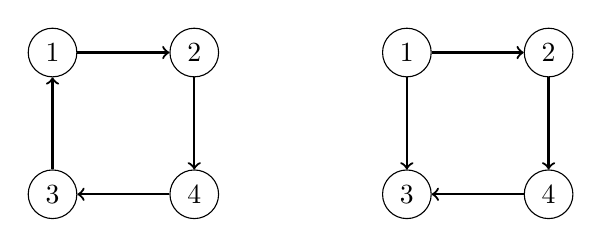
\begin{tikzpicture}[scale=0.9]
        \node[draw, circle] (1) at (1,1) {$1$};
        \node[draw, circle] (2) at (3,1) {$2$};
        \node[draw, circle] (3) at (1,-1) {$3$};
        \node[draw, circle] (4) at (3,-1) {$4$};

        \path[draw,thick,->] (1) -- (2);
        \path[draw,thick,->] (2) -- (4);
        \path[draw,thick,->] (4) -- (3);
        \path[draw,thick,->] (3) -- (1);

        \node[draw, circle] (1b) at (6,1) {$1$};
        \node[draw, circle] (2b) at (8,1) {$2$};
        \node[draw, circle] (3b) at (6,-1) {$3$};
        \node[draw, circle] (4b) at (8,-1) {$4$};

        \path[draw,thick,->] (1b) -- (2b);
        \path[draw,thick,->] (2b) -- (4b);
        \path[draw,thick,->] (4b) -- (3b);
        \path[draw,thick,->] (1b) -- (3b);
    \end{tikzpicture}
\end{center}

El grafo de la derecha no es fuertemente conexo porque, por ejemplo,
no hay un camino desde el nodo 2 al nodo 1.

\index{componente fuertemente conexo}
\index{grafo de componentes}

Los \key{componentes fuertemente conexos} de un grafo lo dividen
en partes que son fuertemente conexas y tan grandes como sea posible.
Los componentes fuertemente conexos forman un \key{grafo de componentes}
acíclico que representa la estructura profunda del grafo original.

Por ejemplo, para el grafo
\begin{center}
    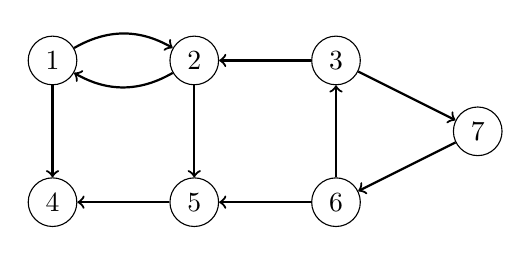
\begin{tikzpicture}[scale=0.9,label distance=-2mm]
        \node[draw, circle] (1) at (-1,1) {$7$};
        \node[draw, circle] (2) at (-3,2) {$3$};
        \node[draw, circle] (4) at (-5,2) {$2$};
        \node[draw, circle] (6) at (-7,2) {$1$};
        \node[draw, circle] (3) at (-3,0) {$6$};
        \node[draw, circle] (5) at (-5,0) {$5$};
        \node[draw, circle] (7) at (-7,0) {$4$};

        \path[draw,thick,->] (2) -- (1);
        \path[draw,thick,->] (1) -- (3);
        \path[draw,thick,->] (3) -- (2);
        \path[draw,thick,->] (2) -- (4);
        \path[draw,thick,->] (3) -- (5);
        \path[draw,thick,->] (4) edge [bend left] (6);
        \path[draw,thick,->] (6) edge [bend left] (4);
        \path[draw,thick,->] (4) -- (5);
        \path[draw,thick,->] (5) -- (7);
        \path[draw,thick,->] (6) -- (7);
    \end{tikzpicture}
\end{center}
los componentes fuertemente conexos son los siguientes:
\begin{center}
    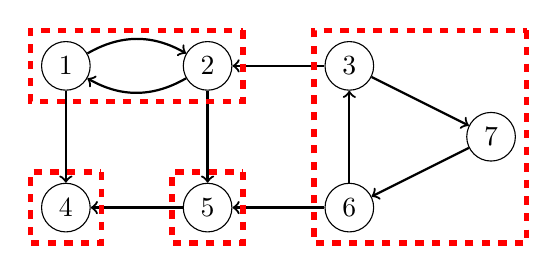
\begin{tikzpicture}[scale=0.9]
        \node[draw, circle] (1) at (-1,1) {$7$};
        \node[draw, circle] (2) at (-3,2) {$3$};
        \node[draw, circle] (4) at (-5,2) {$2$};
        \node[draw, circle] (6) at (-7,2) {$1$};
        \node[draw, circle] (3) at (-3,0) {$6$};
        \node[draw, circle] (5) at (-5,0) {$5$};
        \node[draw, circle] (7) at (-7,0) {$4$};

        \path[draw,thick,->] (2) -- (1);
        \path[draw,thick,->] (1) -- (3);
        \path[draw,thick,->] (3) -- (2);
        \path[draw,thick,->] (2) -- (4);
        \path[draw,thick,->] (3) -- (5);
        \path[draw,thick,->] (4) edge [bend left] (6);
        \path[draw,thick,->] (6) edge [bend left] (4);
        \path[draw,thick,->] (4) -- (5);
        \path[draw,thick,->] (5) -- (7);
        \path[draw,thick,->] (6) -- (7);

        \draw [red,thick,dashed,line width=2pt] (-0.5,2.5) rectangle (-3.5,-0.5);
        \draw [red,thick,dashed,line width=2pt] (-4.5,2.5) rectangle (-7.5,1.5);
        \draw [red,thick,dashed,line width=2pt] (-4.5,0.5) rectangle (-5.5,-0.5);
        \draw [red,thick,dashed,line width=2pt] (-6.5,0.5) rectangle (-7.5,-0.5);
    \end{tikzpicture}
\end{center}
El grafo de componentes correspondiente es el siguiente:
\begin{center}
    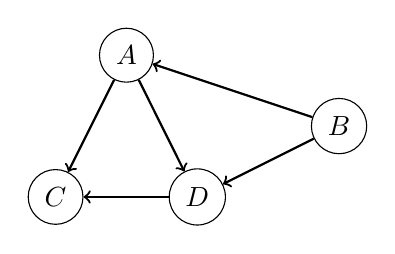
\begin{tikzpicture}[scale=0.9]
        \node[draw, circle] (1) at (-3,1) {$B$};
        \node[draw, circle] (2) at (-6,2) {$A$};
        \node[draw, circle] (3) at (-5,0) {$D$};
        \node[draw, circle] (4) at (-7,0) {$C$};

        \path[draw,thick,->] (1) -- (2);
        \path[draw,thick,->] (1) -- (3);
        \path[draw,thick,->] (2) -- (3);
        \path[draw,thick,->] (2) -- (4);
        \path[draw,thick,->] (3) -- (4);
    \end{tikzpicture}
\end{center}
Los componentes son $A=\{1,2\}$, $B=\{3,6,7\}$, $C=\{4\}$ y $D=\{5\}$.

Un grafo de componentes es acíclico y dirigido, por lo que es más fácil
de procesar que el grafo original. Ya que el grafo no contiene ciclos,
siempre podemos construir un ordenamiento topológico y utilizar
técnicas de programación dinámica como aquellas presentadas en el
Capítulo 16.

\section{Algoritmo de Kosaraju}

\index{algoritmo de Kosaraju}

El \key{algoritmo de Kosaraju}\footnote{Según \cite{aho83},
    S. R. Kosaraju inventó este algoritmo en 1978 pero no lo publicó.
    En 1981, el mismo algoritmo fue redescubierto y publicado por
    M. Sharir \cite{sha81}.} es un eficiente método para encontrar
los componentes fuertemente conexos de un grafo dirigido.
El algoritmo realiza dos búsquedas en profundidad: la primera construye
una lista de nodos según la estructura del grafo, y la segunda forma los
componentes fuertemente conexos

\subsubsection{Búsqueda 1}

La primera fase del algoritmo de Kosaraju construye una lista de nodos
en el orden en que los procesa una búsqueda en profundidad. El algoritmo
recorre los nodos y comienza una búsqueda en profundidad en cada nodo
sin procesar. Cada nodo será añadido a la lista luego de ser procesado.

En el grafo de ejemplo, los nodos son procesados en el siguiente orden:
\begin{center}
    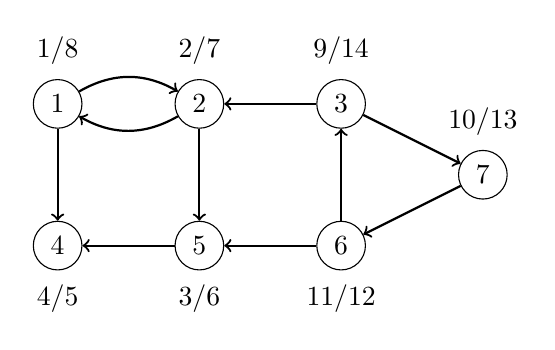
\begin{tikzpicture}[scale=0.9,label distance=-2mm]
        \node[draw, circle] (1) at (-1,1) {$7$};
        \node[draw, circle] (2) at (-3,2) {$3$};
        \node[draw, circle] (4) at (-5,2) {$2$};
        \node[draw, circle] (6) at (-7,2) {$1$};
        \node[draw, circle] (3) at (-3,0) {$6$};
        \node[draw, circle] (5) at (-5,0) {$5$};
        \node[draw, circle] (7) at (-7,0) {$4$};

        \node at (-7,2.75) {$1/8$};
        \node at (-5,2.75) {$2/7$};
        \node at (-3,2.75) {$9/14$};
        \node at (-7,-0.75) {$4/5$};
        \node at (-5,-0.75) {$3/6$};
        \node at (-3,-0.75) {$11/12$};
        \node at (-1,1.75) {$10/13$};

        \path[draw,thick,->] (2) -- (1);
        \path[draw,thick,->] (1) -- (3);
        \path[draw,thick,->] (3) -- (2);
        \path[draw,thick,->] (2) -- (4);
        \path[draw,thick,->] (3) -- (5);
        \path[draw,thick,->] (4) edge [bend left] (6);
        \path[draw,thick,->] (6) edge [bend left] (4);
        \path[draw,thick,->] (4) -- (5);
        \path[draw,thick,->] (5) -- (7);
        \path[draw,thick,->] (6) -- (7);
    \end{tikzpicture}
\end{center}
\newpage
La notación $x/y$ significa que procesar el nodo comenzó al tiempo $x$
y finalizó al tiempo $y$. Por lo tanto, la lista correspondiente
se ve así:
\begin{center}
    \begin{tabular}{ll}
        \\
        nodo & tiempo de procesamiento \\
        \hline
        4    & 5                       \\
        5    & 6                       \\
        2    & 7                       \\
        1    & 8                       \\
        6    & 12                      \\
        7    & 13                      \\
        3    & 14                      \\
        \\
    \end{tabular}
\end{center}
%
% In the second phase of the algorithm,
% the nodes will be processed
% in reverse order: $[3,7,6,1,2,5,4]$.

\subsubsection{Búsqueda 2}

La segunda fase del algoritmo forma los componentes fuertemente conexos
del grafo. Primero, el algoritmo invierte cada arista en el grafo. Esto
garantiza que durante la segunda búsqueda, siempre encontraremos
componentes fuertemente conexos que no contienen nodos extra.

Luego de invertir las aristas, el grafo de ejemplo es el siguiente:
\begin{center}
    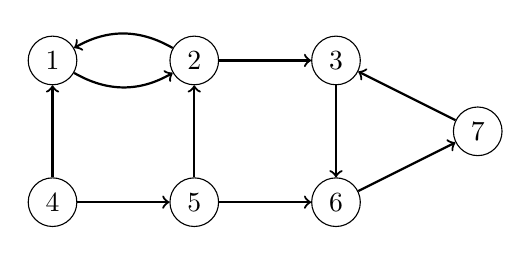
\begin{tikzpicture}[scale=0.9,label distance=-2mm]
        \node[draw, circle] (1) at (-1,1) {$7$};
        \node[draw, circle] (2) at (-3,2) {$3$};
        \node[draw, circle] (4) at (-5,2) {$2$};
        \node[draw, circle] (6) at (-7,2) {$1$};
        \node[draw, circle] (3) at (-3,0) {$6$};
        \node[draw, circle] (5) at (-5,0) {$5$};
        \node[draw, circle] (7) at (-7,0) {$4$};

        \path[draw,thick,<-] (2) -- (1);
        \path[draw,thick,<-] (1) -- (3);
        \path[draw,thick,<-] (3) -- (2);
        \path[draw,thick,<-] (2) -- (4);
        \path[draw,thick,<-] (3) -- (5);
        \path[draw,thick,<-] (4) edge [bend left] (6);
        \path[draw,thick,<-] (6) edge [bend left] (4);
        \path[draw,thick,<-] (4) -- (5);
        \path[draw,thick,<-] (5) -- (7);
        \path[draw,thick,<-] (6) -- (7);
    \end{tikzpicture}
\end{center}
Luego de esto, el algoritmo recorre la lista de nodos creada por la
primera búsqueda en orden \emph{inverso}. Si un nodo no pertenece a
ningún componente, el algoritmo crea un nuevo componente y comienza
una búsqueda en profundidad que añade todos los nuevos nodos
encontrados durante la búsqueda al nuevo componente.

En el grafo de ejemplo, el primer componente comienza en el nodo 3:
\begin{center}
    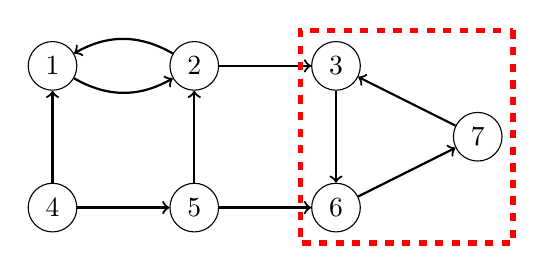
\begin{tikzpicture}[scale=0.9,label distance=-2mm]
        \node[draw, circle] (1) at (-1,1) {$7$};
        \node[draw, circle] (2) at (-3,2) {$3$};
        \node[draw, circle] (4) at (-5,2) {$2$};
        \node[draw, circle] (6) at (-7,2) {$1$};
        \node[draw, circle] (3) at (-3,0) {$6$};
        \node[draw, circle] (5) at (-5,0) {$5$};
        \node[draw, circle] (7) at (-7,0) {$4$};

        \path[draw,thick,<-] (2) -- (1);
        \path[draw,thick,<-] (1) -- (3);
        \path[draw,thick,<-] (3) -- (2);
        \path[draw,thick,<-] (2) -- (4);
        \path[draw,thick,<-] (3) -- (5);
        \path[draw,thick,<-] (4) edge [bend left] (6);
        \path[draw,thick,<-] (6) edge [bend left] (4);
        \path[draw,thick,<-] (4) -- (5);
        \path[draw,thick,<-] (5) -- (7);
        \path[draw,thick,<-] (6) -- (7);

        \draw [red,thick,dashed,line width=2pt] (-0.5,2.5) rectangle (-3.5,-0.5);
    \end{tikzpicture}
\end{center}
Ten en cuenta que ya que todas las aristas están invertidas, el
componente no ``fuga'' a otras partes del grafo.
\newpage
Los siguientes nodos en la lista son los nodos 7 y 6, pero ya pertenecen
a un componente, por lo que el nuevo componente comienza en el nodo 1:
\begin{center}
    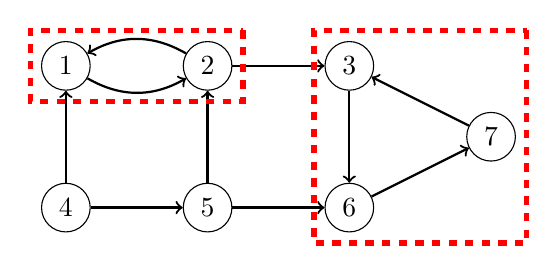
\begin{tikzpicture}[scale=0.9,label distance=-2mm]
        \node[draw, circle] (1) at (-1,1) {$7$};
        \node[draw, circle] (2) at (-3,2) {$3$};
        \node[draw, circle] (4) at (-5,2) {$2$};
        \node[draw, circle] (6) at (-7,2) {$1$};
        \node[draw, circle] (3) at (-3,0) {$6$};
        \node[draw, circle] (5) at (-5,0) {$5$};
        \node[draw, circle] (7) at (-7,0) {$4$};

        \path[draw,thick,<-] (2) -- (1);
        \path[draw,thick,<-] (1) -- (3);
        \path[draw,thick,<-] (3) -- (2);
        \path[draw,thick,<-] (2) -- (4);
        \path[draw,thick,<-] (3) -- (5);
        \path[draw,thick,<-] (4) edge [bend left] (6);
        \path[draw,thick,<-] (6) edge [bend left] (4);
        \path[draw,thick,<-] (4) -- (5);
        \path[draw,thick,<-] (5) -- (7);
        \path[draw,thick,<-] (6) -- (7);

        \draw [red,thick,dashed,line width=2pt] (-0.5,2.5) rectangle (-3.5,-0.5);
        \draw [red,thick,dashed,line width=2pt] (-4.5,2.5) rectangle (-7.5,1.5);
        %\draw [red,thick,dashed,line width=2pt] (-4.5,0.5) rectangle (-5.5,-0.5);
        %\draw [red,thick,dashed,line width=2pt] (-6.5,0.5) rectangle (-7.5,-0.5);
    \end{tikzpicture}
\end{center}
Finalmente, el algoritmo procesa los nodos 5 y 4 que crean los
componentes fuertemente conexos restantes:
\begin{center}
    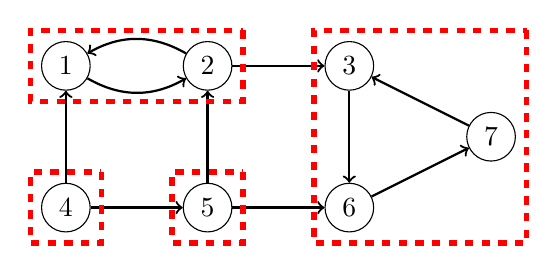
\begin{tikzpicture}[scale=0.9,label distance=-2mm]
        \node[draw, circle] (1) at (-1,1) {$7$};
        \node[draw, circle] (2) at (-3,2) {$3$};
        \node[draw, circle] (4) at (-5,2) {$2$};
        \node[draw, circle] (6) at (-7,2) {$1$};
        \node[draw, circle] (3) at (-3,0) {$6$};
        \node[draw, circle] (5) at (-5,0) {$5$};
        \node[draw, circle] (7) at (-7,0) {$4$};

        \path[draw,thick,<-] (2) -- (1);
        \path[draw,thick,<-] (1) -- (3);
        \path[draw,thick,<-] (3) -- (2);
        \path[draw,thick,<-] (2) -- (4);
        \path[draw,thick,<-] (3) -- (5);
        \path[draw,thick,<-] (4) edge [bend left] (6);
        \path[draw,thick,<-] (6) edge [bend left] (4);
        \path[draw,thick,<-] (4) -- (5);
        \path[draw,thick,<-] (5) -- (7);
        \path[draw,thick,<-] (6) -- (7);

        \draw [red,thick,dashed,line width=2pt] (-0.5,2.5) rectangle (-3.5,-0.5);
        \draw [red,thick,dashed,line width=2pt] (-4.5,2.5) rectangle (-7.5,1.5);
        \draw [red,thick,dashed,line width=2pt] (-4.5,0.5) rectangle (-5.5,-0.5);
        \draw [red,thick,dashed,line width=2pt] (-6.5,0.5) rectangle (-7.5,-0.5);
    \end{tikzpicture}
\end{center}
La complejidad temporal del algoritmo es $O(n+m)$, porque el algoritmo
realiza dos búsquedas en profundidad.

\section{Problema 2SAT}

\index{problema 2SAT}

La conectividad fuerte también está relacionada al \key{problema 2SAT}.
\footnote{El algoritmo presentado aquí fue introducido en \cite{asp79}.
    También hay un algoritmo conocido de tiempo lineal \cite{eve75}
    que se basa en el backtracking.}

En este problema, recibimos una fórmula lógica
\[
    (a_1 \lor b_1) \land (a_2 \lor b_2) \land \cdots \land (a_m \lor b_m),
\]
donde cada $a_i$ y $b_i$ es o una variable lógica
($x_1,x_2,\ldots,x_n$) o la negación de una variable lógica
($\lnot x_1, \lnot x_2, \ldots, \lnot x_n$).
Los símbolos ``$\land$'' y ``$\lor$'' denotan los operadores lógicos
``and'' y ``or''. Nuestra tarea es asignarle a cada variable un
valor tal que la fórmula resulte verdadera, o declarar que esto
no es posible.

Por ejemplo, la fórmula
\[
    L_1 = (x_2 \lor \lnot x_1) \land
    (\lnot x_1 \lor \lnot x_2) \land
    (x_1 \lor x_3) \land
    (\lnot x_2 \lor \lnot x_3) \land
    (x_1 \lor x_4)
\]
es verdadera cuando asignamos los siguientes valores:

\[
    \begin{cases}
        x_1 = \textrm{falso}     \\
        x_2 = \textrm{falso}     \\
        x_3 = \textrm{verdadero} \\
        x_4 = \textrm{verdadero} \\
    \end{cases}
\]

Sin embargo, la fórmula
\[
    L_2 = (x_1 \lor x_2) \land
    (x_1 \lor \lnot x_2) \land
    (\lnot x_1 \lor x_3) \land
    (\lnot x_1 \lor \lnot x_3)
\]
siempre es falsa, independientemente de cómo asignemos los valores.
La razón de esto es que no podemos elegir un valor de $x_1$ sin
crear una contradicción. Si $x_1$ es falso, entonces $x_2$ y
$\lnot x_2$ deben ser falsos, lo que es imposible, y si $x_1$ es
verdadero, entonces $x_3$ y $\lnot x_3$ deben ser verdaderos, que
también es imposible.

El problema 2SAT puede representarse como un grafo cuyos nodos
corresponden a las variables $x_i$ y negaciones $\lnot x_i$, y aristas
determinan las conexiones entre las variables. Cada par $(a_i \lor b_i)$
genera dos aristas: $\lnot a_i \to b_i$ y $\lnot b_i \to a_i$.
Esto significa que si $a_i$ es falso, $b_i$ debe ser verdadero, y
vice versa.

El grafo para la fórmula $L_1$ es:

\begin{center}
    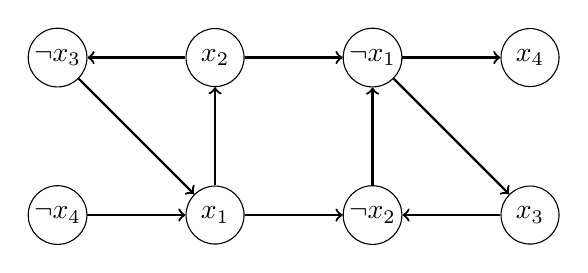
\begin{tikzpicture}[scale=1.0,minimum size=2pt]
        \node[draw, circle, inner sep=1.3pt] (1) at (1,2) {$\lnot x_3$};
        \node[draw, circle] (2) at (3,2) {$x_2$};
        \node[draw, circle, inner sep=1.3pt] (3) at (1,0) {$\lnot x_4$};
        \node[draw, circle] (4) at (3,0) {$x_1$};
        \node[draw, circle, inner sep=1.3pt] (5) at (5,2) {$\lnot x_1$};
        \node[draw, circle] (6) at (7,2) {$x_4$};
        \node[draw, circle, inner sep=1.3pt] (7) at (5,0) {$\lnot x_2$};
        \node[draw, circle] (8) at (7,0) {$x_3$};

        \path[draw,thick,->] (1) -- (4);
        \path[draw,thick,->] (4) -- (2);
        \path[draw,thick,->] (2) -- (1);
        \path[draw,thick,->] (3) -- (4);
        \path[draw,thick,->] (2) -- (5);
        \path[draw,thick,->] (4) -- (7);
        \path[draw,thick,->] (5) -- (6);
        \path[draw,thick,->] (5) -- (8);
        \path[draw,thick,->] (8) -- (7);
        \path[draw,thick,->] (7) -- (5);
    \end{tikzpicture}
\end{center}

Y el grafo para la fórmula $L_2$ es:

\begin{center}
    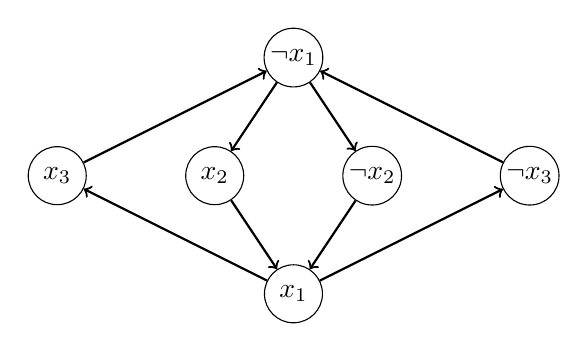
\begin{tikzpicture}[scale=1.0,minimum size=2pt]
        \node[draw, circle] (1) at (1,2) {$x_3$};
        \node[draw, circle] (2) at (3,2) {$x_2$};
        \node[draw, circle, inner sep=1.3pt] (3) at (5,2) {$\lnot x_2$};
        \node[draw, circle, inner sep=1.3pt] (4) at (7,2) {$\lnot x_3$};
        \node[draw, circle, inner sep=1.3pt] (5) at (4,3.5) {$\lnot x_1$};
        \node[draw, circle] (6) at (4,0.5) {$x_1$};

        \path[draw,thick,->] (1) -- (5);
        \path[draw,thick,->] (4) -- (5);
        \path[draw,thick,->] (6) -- (1);
        \path[draw,thick,->] (6) -- (4);
        \path[draw,thick,->] (5) -- (2);
        \path[draw,thick,->] (5) -- (3);
        \path[draw,thick,->] (2) -- (6);
        \path[draw,thick,->] (3) -- (6);
    \end{tikzpicture}
\end{center}

La estructura del grafo nos dice si es posible asignar los valores
a las variables tal que la fórmula sea verdadera. Resulta
que esto es posible solo cuando no hay nodos $x_i$ y $\lnot x_i$
tal que estos dos no pertenezcan al mismo componente fuertemente conexo.
Si es así, el grafo contiene un camino de $x_i$ a
$\lnot x_i$ y también un camino de $\lnot x_i$ a $x_i$, por lo que
$x_i$ y $\lnot x_i$ deben ser verdaderos, que es imposible.

En el grafo de la fórmula $L_1$ no existen nodos $x_i$ y $\lnot x_i$
tal que ambos nodos pertenezcan al mismo componente fuertemente conexo,
así que una solución existe. En el grafo de la fórmula $L_2$ todos los
nodos pertenecen al mismo componente fuertemente conexo, así que una
solución no existe.

Si una solución existe, los valores de las variables pueden encontrarse
si recorremos los nodos del grafo de componentes en ordenamiento
topológico inverso. En cada paso, procesamos un componente que no
contenga aristas que lleven hacia un componente sin procesar.
Si las variables en el componente no han sido asignadas valores,
sus valores serán determinados acorde a los valores en el componente,
y si ya tienen valores, quedarán sin cambiar. El proceso continúa hasta
que cada variable haya sido asignada un valor.

\newpage
El grafo de componentes para la fórmula $L_1$ es el siguiente:
\begin{center}
    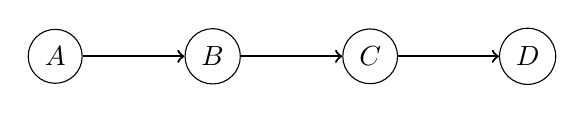
\begin{tikzpicture}[scale=1.0]
        \node[draw, circle] (1) at (0,0) {$A$};
        \node[draw, circle] (2) at (2,0) {$B$};
        \node[draw, circle] (3) at (4,0) {$C$};
        \node[draw, circle] (4) at (6,0) {$D$};

        \path[draw,thick,->] (1) -- (2);
        \path[draw,thick,->] (2) -- (3);
        \path[draw,thick,->] (3) -- (4);
    \end{tikzpicture}
\end{center}

Los componentes son
$A = \{\lnot x_4\}$,
$B = \{x_1, x_2, \lnot x_3\}$,
$C = \{\lnot x_1, \lnot x_2, x_3\}$ y
$D = \{x_4\}$. Cuando construimos una solución, primero procesamos el
componente $D$ donde $x_4$ se vuelve verdadero. Luego de esto,
procesamos el componente $C$ donde $x_1$ y $x_2$ se vuelven falsos y
$x_3$ se vuelve verdadero. Todas las variables han sido asignadas
valores, así que los componentes restantes $A$ y $B$ no modifican
las variables.

Ten en cuenta que este método funciona porque el grafo tiene una
estructura especial: si existen caminos del nodo $x_i$ al nodo $x_j$
y del nodo $x_j$ al nodo $\lnot x_j$, entonces el nodo $x_i$ nunca se
vuelve verdadero. La razón es que también existe un camino
desde el nodo $\lnot x_j$ al nodo $\lnot x_i$, y $x_i$ y $x_j$ se
vuelven falsos.

\index{problema 3SAT}

Un problema más difícil es el \key{problema 3SAT}, donde cada parte
de la fórmula tiene la forma $(a_i \lor b_i \lor c_i)$. Este problema es
NP-difícil, ya que no se conoce un algoritmo eficiente para resolverlo.
